\section{Шифрование файлов и почтовых сообщений в PGP}
\selectlanguage{russian}

В качестве примера передачи файлов по сети с обеспечением аутентификации, конфиденциальности и целостности рассмотрим систему PGP (Pretty Good Privacy), разработанную Филом Циммерманном (Phil Zimmermann) в 1991 г. Изначально система предлагалась к использованию для защищенной передачи электронной почты. Стандартом PGP является OpenPGP. Примерами реализации стандарта OpenPGP являются GNU Privacy Guard (GPG) и netpgp, разработанные в рамках проектов GNU и NetBSD соответственно.

Каждый пользователь обладает одним или несколькими закрытыми ключами для криптосистемы с открытым ключом, которые используются для аутентификации посредством ЭП. Пользователь хранит также открытые ключи других пользователей, которые он использует для шифрования секретного сеансового ключа блокового шифрования. Передаваемое сообщение подписывается секретным ключом отправителя, затем сообщение шифруется блоковой криптосистемой на случайно выбранном сеансовом ключе. Сам сеансовый ключ шифруется криптосистемой с открытым ключом на открытом ключе получателя.

Свои закрытые ключи отправитель хранит в зашифрованном виде. Набор ключей называется связкой закрытых ключей. Шифрование закрытых ключей в связке производится симметричным шифром\index{шифр!симметричный}, ключом которого является функция от пароля, вводимого пользователем. Шифрование закрытых ключей, хранимых на компьютере, является стандартной практикой для защиты от утечки, например, в случае взлома ОС, утери ПК и т.~д.

Набор открытых ключей других пользователей называется связкой открытых ключей.

\begin{figure}[!ht]
	\centering
	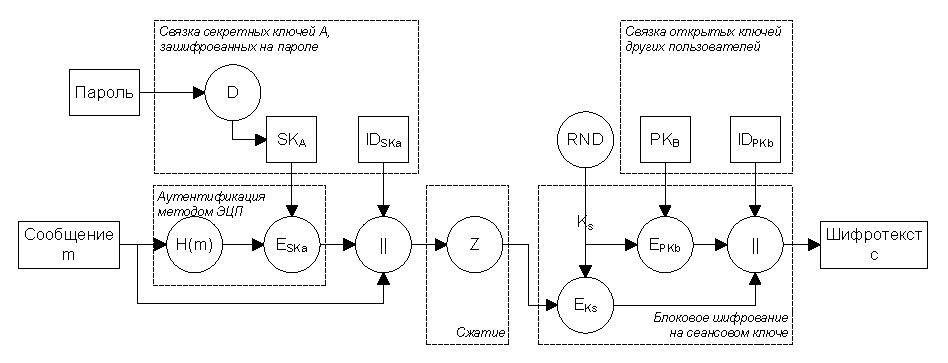
\includegraphics[width=0.9\textwidth]{pic/pgp}
	\caption{Схема обработки сообщения в PGP\label{fig:pgp}}
\end{figure}

На рис.~\ref{fig:pgp} представлена схема обработки сообщения в PGP для передачи от $A$ к $B$. Использование аутентификации, сжатия и блокового шифрования является опциональным. Обозначения на рисунке следующие.
\begin{itemize}
    \item Пароль -- пароль, вводимый отправителем для расшифрования связки своих закрытых ключей.
    \item $D$ -- расшифрование блоковой криптосистемы для извлечения секретного ключа ЭП отправителя.
    \item $SK_A$ -- закрытый ключ ЭП отправителя.
    \item $ID_{SKa}$ -- идентификатор ключа ЭП отправителя, по которому получатель определяет, какой ключ из связки открытых ключей использовать для проверки подписи.
    \item $m$ -- сообщение (файл) для передачи.
    \item $h(m)$ -- криптографическая хэш-функция.
    \item $E_{SKa}$ -- схема ЭП на секретном ключе $SK_A$.
    \item $\|$ -- конкатенация битовых строк.
    \item $Z$ -- сжатие сообщения алгоритмом компрессии.
    \item $RND$ -- криптографический генератор псевдослучайной последовательности.
    \item $K_s$ -- сгенерированный псевдослучайный сеансовый ключ.
    \item $E_{Ks}$ -- блоковое шифрование на секретном сеансовом ключе $K_s$.
    \item $PK_B$ -- открытый ключ получателя.
    \item $ID_{PKb}$ -- идентификатор открытого ключа получателя, по которому получатель определяет, какой ключ из связки закрытых ключей использовать для расшифрования сеансового ключа.
    \item $E_{PKb}$ -- шифрование сеансового ключа криптосистемой с открытым ключом на открытом ключе $B$.
    \item $c$ -- зашифрованное подписанное сообщение.
\end{itemize}
